% !TeX spellcheck = <none>
\documentclass[10pt,twocolumn,letterpaper,english]{article}

\usepackage{cvpr}
\usepackage{times}
\usepackage{epsfig}
\usepackage{graphicx}
\usepackage{amsmath}
\usepackage{amssymb}
\usepackage{listings}

\lstdefinestyle{compactcode}{
	basicstyle=\small\ttfamily,
	breaklines=true,
	showstringspaces=false,
	breakatwhitespace=true,
	breakindent=0pt,
	escapeinside={(*@}{@*)},
	frame=single,
	aboveskip=2pt,
	belowskip=2pt
}

\usepackage{url}

% Include other packages here, before hyperref.

% If you comment hyperref and then uncomment it, you should delete
% egpaper.aux before re-running latex.  (Or just hit 'q' on the first latex
% run, let it finish, and you should be clear).
\usepackage[pagebackref=true,breaklinks=true,letterpaper=true,colorlinks,bookmarks=false]{hyperref}

\cvprfinalcopy % *** Uncomment this line for the final submission

\def\cvprPaperID{****} % *** Enter the CVPR Paper ID here
\def\httilde{\mbox{\tt\raisebox{-.5ex}{\symbol{126}}}}

% Pages are numbered in submission mode, and unnumbered in camera-ready
\ifcvprfinal\pagestyle{empty}\fi
\begin{document}

%%%%%%%%% TITLE
\title{PC-2023/24 Alpha-Compositor}

\author{Christian Mancini\\
E-mail address\\
{\tt\small christian.mancini1@edu.unifi.it}
% For a paper whose authors are all at the same institution,
% omit the following lines up until the closing ``}''.
% Additional authors and addresses can be added with ``\and'',
% just like the second author.
% To save space, use either the email address or home page, not both
}

\maketitle
\thispagestyle{empty}

%%%%%%%%% ABSTRACT
\begin{abstract}
We implement a parallel version of the alpha compositor, to compose a foreground over multiples  background in a fixed position, starting from a serial version. We also show the speed up we gained of just the compositing part and the overall program with 12 and 7 times of speed up respectively. The tests were made on an Arch Laptop with Linux Kernel 6.7.9, 11th Gen Intel(R) Core(TM) i7-11800H @ 2.30GHz 8 cores 16 threads,  23 GB of dual Channel 3200MHz RAM (16 + 8) and max memory bandwidth 51.2 GB/s.
\end{abstract}

%%%%%%%%% BODY TEXT
\noindent\large\textbf{Future Distribution Permission}\\
\indent The author(s) of this report give permission for this document to be distributed to Unifi-affiliated students taking future courses.

\section{Introduction}

Alpha compositing or alpha blending is the process of combining one image with a background to create the appearance of partial or full transparency. In a 2D image a color combination is stored for each picture element (pixel), often a combination of red, green and blue (RGB). When alpha compositing is in use, each pixel has an additional numeric value stored in its alpha channel (RGBA), with a value ranging from 0 to 1. A value of 0 means that the pixel is fully transparent and the color in the pixel beneath will show through. A value of 1 means that the pixel is fully opaque. 
With this definition in mind we can produce the effect of drawing the
source pixels on top of the destination pixels (foreground over a background) using the following formula: 
\begin{equation}\label{eq:composting}
	[RGBA]_d = [RGBA]_s + [RGBA]_d(1-A_s)
\end{equation}
For our scope the foreground must be completely opaque. Changing the weights leads to different results. 

%-------------------------------------------------------------------------
\subsection{Compositing Algorithm}

The compositing algorithm is straightforward, we just need to apply the \ref{eq:composting} on every channel of the background image.
\begin{lstlisting}[style=compactcode, language=C]

for (int color = 0; color < 3; ++color) {
	background.rgb_image[backgroundIndex + color] =
	background.rgb_image[backgroundIndex + color] * beta
	+ foreground.rgb_image[foregroundIndex + color] * alpha;
}

\end{lstlisting}

This is just a snippet of the compose function.
%-------------------------------------------------------------------------

The program has to performe 3 simple tasks:
\begin{enumerate}
	\item Read Foreground and a vector of Backgrounds;
	\item Compose Foreground on every Background;
	\item Save all the Backgrounds on disk.
\end{enumerate}
The most expensive operation is as expected the last one.

\begin{figure*}[htbp]
	\centering
	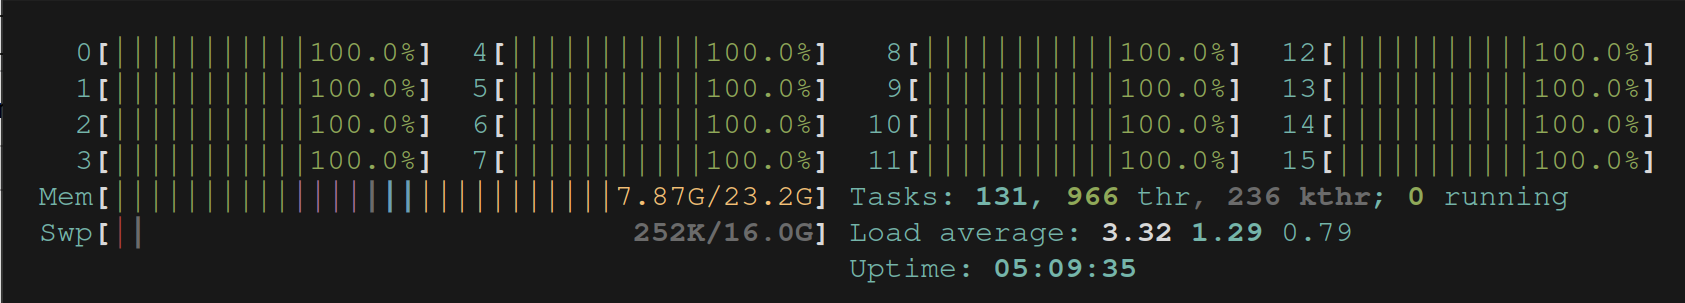
\includegraphics[width=\textwidth]{Threads.png}
	\caption{All cores are working}
	\label{fig:Cores}
\end{figure*}
\section{Parallelization Criteria}
There are many ways to parallelize a program. The first step we take is to us Vallgrid \cite{valgrind} to check that we don't have leaks in the serial version of the program.

We can now decide how to parallelize the program using OpenMP \cite{openmp}.
Since we are dealing with small images, parallelize the compositing function will lead a slower computing time, instead we let each thread to call its own compositing function to a defined image. Loading and Saving follows the same idea.
We got the following results:
\begin{table}[htbp]
	\centering
	\begin{tabular}{|l|c|c|c|c|}
		\hline
		& Load & Compose & Save & Total\\
		\hline
		Serial & 0.57s & 0.77s & 40.78s & 42,13s\\
		Parallel & 0.32s & 0.058s & 5,90s & 6.29s\\
		\hline
	\end{tabular}
	\caption{256x256 Foreground and 513 Backgrounds (roughly same dimention of foreground ).}
	\label{tab:Mesurements}
\end{table}
\begin{table}[htbp]
	\centering
	\begin{tabular}{|l|c|}
		\hline
		Fase & Speedup \\
		\hline
		Load & $ \approx 1.78$ \\
		Compose & $ \approx 13.28$ \\
		Save & $\approx 6.91$ \\
		Total & $\approx 6.70$ \\
		\hline
	\end{tabular}
	\caption{Speedup.}
	\label{tab:Speedup}
\end{table}
We can see from figure \ref*{fig:Cores} that all the cores are woking during the parallel execution.



{\small
\bibliographystyle{ieee}
\bibliography{egbib}
}


\end{document}
